\documentclass[letterpaper,12pt,oneside]{book}

\usepackage[utf8]{inputenc}
\usepackage[spanish,es-nodecimaldot,es-tabla]{babel}
\usepackage{graphicx}
\usepackage{natbib}  % Usando paquete para citas
\usepackage{amsmath} % Notación
\usepackage{amssymb}
\usepackage{amsthm}  % Definiciones
\usepackage{longtable}

\graphicspath{{./img/}}

\newtheorem{definition}{Definición}

\begin{document}
\bibliographystyle{acl_natbib}  % Cargando estilo de bibliografia

\author{Diego Alberto Barriga Martínez}
\title{Etiquetador automático de la morfología del otomí usando predicción estructurada}
\tableofcontents
\maketitle

\chapter{Introducción}

\section{Problemática}

\subsection{Lengua otomí}

En esta sección se menciona los lugares donde se describe el idioma otomí de forma somera, se mencionan algunos lugares donde es hablado el otomí y características fundamentales de la lengua.

\subsection{Origen}

% Pie de pagina, no meter cosas tangenicales. Citar esta definicion
La palabra otomí es de origen náhuatl (singular: \textit{otomitl}, plural: \textit{otomí}). Por otra parte, los otomíes se nombran a sí mismos \textit{ñähñu}\footnote{Existen organizaciones indígenas, como el Consejo de la Nacionalidad Otomí, que escriben la auto-denominación como hñätho hñähñu y también ñätho ñähño. Sin embargo, esta auto denominación puede variar.}, que significa "los que hablan otomí".

Los grupos indígenas que hablan el idioma otomí se encuentran en diversas partes del territorio mexicano como: Estado de México, Querétaro, Hidalgo, Puebla y Veracruz \citep{barrientos2004otomies}. El otomí es una lengua indígena una gran variación dialectal que depende de su distribución geográfica.

En el Estado de México el pueblo \textit{ñähñu} está disperso por varios municipios tales como: Toluca, Lerma, Chapa de Mota, Aculco, Amanalco, Atizapán de Zaragoza, por mencionar algunos. En otros municipios como Naucalpan, Ecatepec, Nezahualcóyotl y Tlalnepantla se pueden encontrar hablantes por efectos de la migración. Según \citet{barrientos2004otomies} la población total de hablantes otomíes en el Estado de México supera los cien mil, sin embargo, datos actuales .

En concreto existen \textbf{nueve} variantes del otomí y cabe recalcar que dicha variación puede presentarse incluso dentro del mismo estado. Tan solo el Estado de México presenta tres variantes del otomí: El otomí de Tilapa, hablado en el municipio de Santiago Tianguistenco; el Otomí de Acazulco, del municipio de San Jerónimo Acazulco; y el Otomí de Toluca, de San Andrés Cuexcontitlán.

\section{Objetivo}

\section{Hipótesis}

\chapter{Avances en etiquetadores automáticos}

\section{Marco teórico}

\section{Estado del arte}

\section{Los límites de los modelos gráficos}

En este capítulo se explicará qué ventajas tienen los \emph{Conditional Random Fields (CRF)} sobre otros modelos de aprendizaje, se mencionan formalmente los elementos fundamentales que describen los \emph{CRF's}.

En lingüística computacional una tarea de interés es el procesamiento estadístico del lenguaje natural, en particular, el etiquetado y segmentación de secuencias de datos. En ese sentido, es habitual la utilización de \textbf{modelos generativos}, cómo los \textit{Hidden Markov Models (HMMs)}, o \textbf{modelos condicionales}, como los \textit{Maximum Entropy Markov Models (MEMMs)}.

Por una parte, los modelos generativos intentan modelar una probabilidad conjunta $P(x,y)$ sobre observaciones y etiquetas. Para definir esta probabilidad conjunta se necesita enumerar todas las observaciones posibles. Las limitantes de este enfoque son de diversas índoles como las grandes dimensionalidades en el vector de entrada $X$, la dificultad de representar múltiples características que interactúan unas con otras y dependencias complejas que hacen la construcción de la distribución de probabilidad un problema intratable con un enfoque computacional.

Por otro lado, una solución a las limitantes de los modelos generativos es un modelo condicional. Estos modelos no son tan estrictos como los primeros al momento de asumir independencias en las observaciones. Los modelos condicionales especifican la probabilidad de posibles etiquetas dada una secuencia de observación.

Consecuencia de lo anterior, no se gasta esfuerzo en modelar las observaciones, dado que en al momento de realizar pruebas estas observaciones son fijas. Segundo, la probabilidad condicional puede depender de características arbitrarias y no dependientes de la secuencia de observación sin forzar al modelo a tomar en cuenta la distribución de estas características, permitiendo que el modelo sea tratable \citep{lafferty2001conditional}.

Un ejemplo de estas ventajas con los \textit{MEMMs} que son modelos secuenciales de probabilidad condicional. Sin embargo, estos modelos y otros que son no generativos, de estados finitos y que son clasificadores basados en el estado siguiente comparten una debilidad llamada \emph{label bias problem}. \citet{lafferty2001conditional} define que existe el \emph{label bias problem} cuando "las transiciones que dejan un estado compiten solo entre sí, en lugar de entre todas las demás transiciones en el modelo".

Dado que las transiciones son las probabilidades condicionales de los siguientes posibles estados una observación puede afectar cuál será el estado siguiente sin tomar en cuenta que tan adecuado será este. Por tanto, se tendrá un sesgo en los estados con menos transiciones de salida.


\section{Conditional Random Fields}

Como menciona \citet{sutton2012introduction} modelar las dependencias entre las entrada puede conducir a modelos intratables, pero ignorar estas dependencias puede reducir el rendimiento.

Dado el que problema abordado en este trabajo, dónde se requiere del etiquetado de secuencias y es en contexto de bajos recursos lingüísticos, se hace necesario utilizar un enfoque más conveniente.

Los \textit{Conditional Random Fields (CRFs)} son un framework para la creación de modelos probabilístico utilizado en técnicas de aprendizaje estructurado. Tienen las ventajas de los \textit{MEMMs} y, en principio, solucionan el \emph{label bias problem}. El framework tiene un solo modelo exponencial para la probabilidad conjunta de todas las secuencias de las etiquetas de salida dada la secuencia de observación. En contraste los \emph{MEMMs} usan modelos exponenciales para cada probabilidad condicional de los estados siguientes dado el estado actual.

Formalmente \citet{lafferty2001conditional} definen los \textit{CRFs} como a continuacion se enuncia:

\begin{definition}
	Sea $G = (V,E)$ una gráfica tal que $\mathbf{Y} = (\mathbf{Y}_{v})_{v \in V}$, entonces esa $\mathbf{Y}$ es indexada por los vertices de $G$. Entonces $(\mathbf{X}, \mathbf{Y})$ es un \textsf{conditional random field} en caso de que las variables aleatorias $\mathbf{Y}$ se condicionen por $\mathbf{X}$, la variable aleatoria $\mathbf{Y}_{v}$ cumple la \textit{propiedad de Markov} con respecto a la gráfica: $p(\mathbf{Y}_{v}|\mathbf{X},\mathbf{Y}_{w},w \ne v) = p(\mathbf{Y}_{v}|\mathbf{X},\mathbf{Y}_{w},w \sim v)$, dónde $w \sim v$ significa que $w$ y $v$ son vecinos en $G$.
\end{definition}

En esta tesis, para el modelado de secuencias, se utiliza la forma más sencilla de la gráfica $G$ dónde es una cadena simple o línea. Esto quiere decir que $G = (V = \{1,2,...m\}, E = \{(i,i+1)\})$. A este tipo de \textit{CRFs} se les conoce como \textit{linear-chain CRFs}. Como menciona \citet{lafferty2001conditional} "si la gráfica $G = (V,E)$ de $\mathbf{Y}$ es un árbol (del cual una cadena es el ejemplo más sencillo), los cliques??? son los límites y vertices. Entonces, por el teorema de los \textit{random fields} \citep{hammersley1971markov}, la distribución conjunta sobre las etiquetas de secuencias $\mathbf{Y}$ y $\mathbf{X}$ tiene la forma: "


% TODO: Poner tag
\begin{equation}
p{_{\theta}}(y|x) \propto \exp \bigg( \sum\limits_{e \in \mathbf{E},k} \lambda_{k}f_{k}(e,\mathbf{y}|_{e},\mathbf{x}) + \sum\limits_{v \in \mathbf{V},k}\mu_{k}g_{k}(v,\mathbf{y}|_{v},\mathbf{x}) \bigg)
\end{equation}

% TODO: Mencionar la ecucacion

De la ecuación  se destacan $f_{k}$ y $g_{k}$ que representan las \textit{feature functions}. Estas están definidas y son fijas. Las \textit{feature functions} de está tesis serán descritas más adelante. % TODO: Descripcion de la estimacion de parametros y caracteristica de la funcion de perdida


Los \textit{CRFs} han sido utilizados para la clasificación de regiones en una imagen, estimar el puntaje en un juego de Go, segmentar genes en una hebra de ADN y análisis sintáctico de lenguaje natural en un texto por mencionar algunas \citep{sutton2012introduction}.

\chapter{Etiquetador morfológico para el otomí (Metodología)}

En este capitulo se describe el corpus utilizado en este trabajo, se mostrará la arquitectura propuesta para la generación automática de glosa para el idioma otomi. Adicionalmente, se explicará el diseño e implementación del \textit{pipeline} que incluye, entre otras cosas, la determinación de las \textit{feature functions}.

%TODO: Descripcion de la estimacion de parametros y caracteristica de la funcion de perdida

\section{Conditional Random Fields para low resources}

Los CRFs muestran claras ventajas sobre otros métodos de aprendizaje basados en gráficas. Su habilidad de tomar las virtudes de los modelos generativos y de los modelos condicionales presentan a este \textit{framework} como una opción para el contexto de \textit{low resouces} que nos impone, como se describirá más adelante, el tamaño del corpus.
 

% Particularidades del corpus (Analisis cualitativo y cuantitativo)
\section{Corpus: otomí de Toluca}

% Otomi en general, Familia y rama
En este trabajo se utilizará un corpus en otomí que, además, cumple la característica de estar glosado. Se trabaja con la variante del otomí de Toluca de la región de San Andrés Cuexcontitlan. A continuación, una descripción de sus características principales.

% Tipo de otomi y caracteristicas de la variante
La clasificación lingüística introduce al otomí dentro de las lenguas otomianas, las cuales a su vez pertenecen a la rama otopame de la familia otomangue \citep{barrientos2004otomies}. Cada variante muestra particularidades fonológicas, morfológicas, sintácticas y léxicas. En el tratamiento de textos por medio de técnicas de \textit{NLP} se requiere que estos estén normalizados y homogéneos. Lo anterior propicia la obtención del mejor desempeño posible en los diversos métodos de aprendizaje automático. 

% De donde vienen los textos, quien lo glosa y quien lo recolecta
Esta tesis recoge un corpus basado en el trabajo de \citet{lastra1992otomi} titulado \textbf{El otomí de Toluca} y que a su vez es etiquetado y glosado manualmente por el lingüista Víctor Germán Mijangos de la Cruz (TODO: Liga al repositorio). Este corpus es un subconjunto del corpus que se encuentra en la plataforma web Tsunkua (Elotl, 2019) TODO: ¿Como se cita?. El corpus está conformado de los siguientes textos:

\begin{center}
	\begin{tabular}{ c | c }
		Textos narrativos & 32 \\
		Textos dialogados & 4  \\ \hline
		\textbf{Número de textos}  & 36 \\
	\end{tabular}
\end{center}

Los textos que componen el corpus fueron construidos a partir de las aportaciones de diez hablantes distintos de entre diez y setenta y tres años, de los cuales, siete son de sexo femenino y tres masculino \citep{lastra1992otomi}. 
% Caracteristicas escenciales que tiene que ver con el etiquetado POS de las lenguas otomies

% Descripcion detalla del etiquetado POS
% Grafica de Zipf para las etiquetas POS
% Distribucion de etiquetas

% Descripcion del corpus (tipos, tokens)
\subsection{Tipos}

\subsubsection{Etiquetas POS}

\begin{center}
	\begin{tabular}{| c | c | c | c | c |}
		\hline
		v & obl & det & cnj & dem \\ 
		unkwn & n & neg & p.loc & prt \\
		conj.adv & dim & gen & cond & it \\
	    lim & aff & loc & pascuala & toluca \\
	    chente & dec & conj & chalma & mexico \\
	    tapanco & cord & san & cnj.adv & regular/v \\
	    adv & juan & andrés & buena.vista & nada.más \\
	    zapata & calvario & bautisterio & adj & cristo \\
	    emilio & pato & luis & mextepec & \\
	    \hline
	\end{tabular}
\end{center}

\subsubsection{Glosa}

\begin{center}
	\begin{tabular}{| c | c | c | c | c | c | c |}
		\hline
			stem & det & 3.cpl & psd & lim & prag & 3.icp \\

			det.pl & 1.icp & 3.pot & ctrf & 1.pot & pl.exc & 1.cpl \\

			dem & 1.pss & dim & pl & 1.obj & ila & 2.icp \\

			1.prf & 3.cnt & 3.obj & loc & mod & 1.cnt & 3.pls \\

			muy & prt & it & dual.exc & 3.prf & 3.icp.irr & 3.pss \\

			2.pss & 1.enf & med & dual & p.loc & 2.cnt & 2 \\

			3.imp & int & neg & 1.icp.irr & 1.cpl.irr & 2.obj & pues \\

			que & aum & 1.pls & y & 2.cpl & toluca & 2.prf \\

			aqui & gen & hasta & com & 2.pot & adj & cuando \\

			cond & como & 3.cpl.irr & 1.sg & encl & por.que & solo \\

			agujerear/v & mientras & 3.sg & uno & 3.pss.pl & spt & mexico \\

			1.irr & mucho & 2.enf & conj.adv & pueblo & animal.de.dios & caus \\

			tiempo & con & lugar/v & chico & eh & para & comp \\

			prf & dónde & dist & mov & pascuala & 3.irr & loco \\

			coraje & si & det.dem & dcl & nom & chente & vez \\

			rapido & maria & 2.icp.irr & tal.vez & mujer/v & dios & lig \\
		\hline
	\end{tabular}
\end{center}

\subsubsection{Bio-Labels}

\begin{center}
	\begin{longtable}{| c | c | c | c | c | c |}
		\hline
		I-stem & B-stem & I-det & I-lim & B-det & I-det.pl \\

		I-dem & B-3.cpl & I-3.cpl & B-psd & B-lim & I-prag \\

		B-prag & B-3.icp & B-lig & I-dim & B-det.pl & B-1.icp \\

		I-1.icp & I-ila & B-3.pot & I-3.pot & B-ctrf & I-ctrf \\

		B-1.pot & I-1.pot & B-pl.exc & I-pl.exc & B-1.cpl & I-1.cpl \\

		B-dem & I-1.cnt & I-pl & B-1.pss & I-1.pss & I-muy \\

		I-3.cnt & I-loc & B-dim & I-mod & B-pl & B-1.obj \\

		I-1.obj & B-ila & B-2.icp & I-2.icp & B-1.prf & I-1.prf \\

		B-3.cnt & I-prt & I-3.obj & B-3.obj & B-loc & B-mod \\

		B-1.cnt & I-3.pss & B-3.pls & I-3.pls & B-muy & B-prt \\

		I-toluca & B-it & I-it & B-dual.exc & I-dual.exc & B-3.prf \\

		I-3.prf & B-3.icp.irr & I-3.icp.irr & I-2.cnt & B-3.pss & I-3.imp \\

		B-2.pss & I-2.pss & I-neg & I-1.icp.irr & B-1.enf & I-1.enf \\

		B-med & B-dual & I-dual & I-2.obj & I-aum & B-p.loc \\

		I-p.loc & B-2.cnt & B-2 & I-2 & I-int & B-3.imp \\

		B-int & B-neg & B-1.icp.irr & B-1.cpl.irr & I-1.cpl.irr & B-2.obj \\

		I-3.icp & I-gen & I-aqui & B-pues & I-pues & B-que \\

		I-que & B-aum & B-1.pls & I-1.pls & B-y & B-2.cpl \\

		I-2.cpl & I-3.cpl.irr & I-1.sg & I-agujerear/v & I-mientras & B-toluca \\

		B-2.prf & I-2.prf & I-mexico & I-pueblo & I-animal.de.dios & B-aqui \\

		B-gen & B-hasta & I-hasta & I-3.sg & B-com & I-com \\

		I-pascuala & I-solo & I-mucho & I-tiempo & I-cuando & I-chente \\

		I-mujer/v & I-lugar/v & I-chico & I-cond & I-3.pss.pl & I-por.que \\

		I-1.irr & I-maria & B-2.pot & I-2.pot & B-adj & I-adj \\

		B-cuando & B-cond & B-como & I-como & B-3.cpl.irr & B-1.sg \\

		B-encl & I-encl & B-por.que & B-solo & I-loco & I-coraje \\

		B-agujerear/v & I-det.dem & B-mientras & I-con & B-3.sg & I-lig \\

		B-uno & I-uno & B-3.pss.pl & B-spt & I-spt & B-mexico \\

		B-1.irr & B-mucho & I-dcl & B-2.enf & I-2.enf & B-conj.adv \\

		I-vez & I-2.icp.irr & B-pueblo & I-dios & B-animal.de.dios & B-caus \\

		I-caus & B-tiempo & B-con & B-lugar/v & B-chico & B-eh \\

		I-eh & B-para & I-para & B-comp & I-comp & B-prf \\

		I-prf & B-dónde & B-dist & I-dist & B-mov & I-mov \\

		I-med & B-pascuala & B-3.irr & I-3.irr & B-loco & B-coraje \\

		B-si & I-si & I-y & B-det.dem & B-dcl & B-nom \\

		I-nom & B-chente & B-vez & B-rapido & I-rapido & B-maria \\

		B-2.icp.irr & B-tal.vez & I-tal.vez & B-mujer/v & B-dios & 
\\
		\hline
	\end{longtable}
\end{center}

\subsection{Tokens}

\subsubsection{Etiquetas POS}

\begin{center}
	\begin{tabular}{c | c}
		\textbf{Etiqueta} & \textbf{tokens} \\ \hline \hline
		v & 2596 \\

		obl & 2447 \\

		det & 975 \\

		cnj & 837 \\

		dem & 543 \\

		unkwn & 419 \\

		n & 273 \\

		neg & 178 \\

		p.loc & 81 \\

		prt & 49 \\

	\end{tabular}

\end{center}

\subsubsection{Glosa}

\begin{center}
	\begin{tabular}{c | c}                            
		\textbf{Etiqueta} & \textbf{tokens} \\ \hline \hline
		stem & 7527 \\

		det & 733 \\

		3.cpl & 450 \\

		psd & 418 \\

		lim & 374 \\

		prag & 362 \\

		3.icp & 346 \\

		lig & 289 \\

		det.pl & 271 \\

		1.icp & 270 \\
	\end{tabular}

\end{center}

\subsubsection{Bio-Labels}
\begin{center}
	\begin{tabular}{c | c}
		\textbf{Etiqueta} & \textbf{tokens} \\ \hline \hline
		I-stem & 21934 \\

		B-stem & 7527 \\

		I-det & 1469 \\

		I-lim & 1092 \\

		B-det & 733 \\

		I-det.pl & 553 \\

		I-dem & 485 \\

		B-3.cpl & 450 \\

		I-3.cpl & 450 \\

		B-psd & 418 \\

	\end{tabular}
\end{center}

\subsection{Distribución de etiquetas}

\begin{figure}[h]
	\centering
	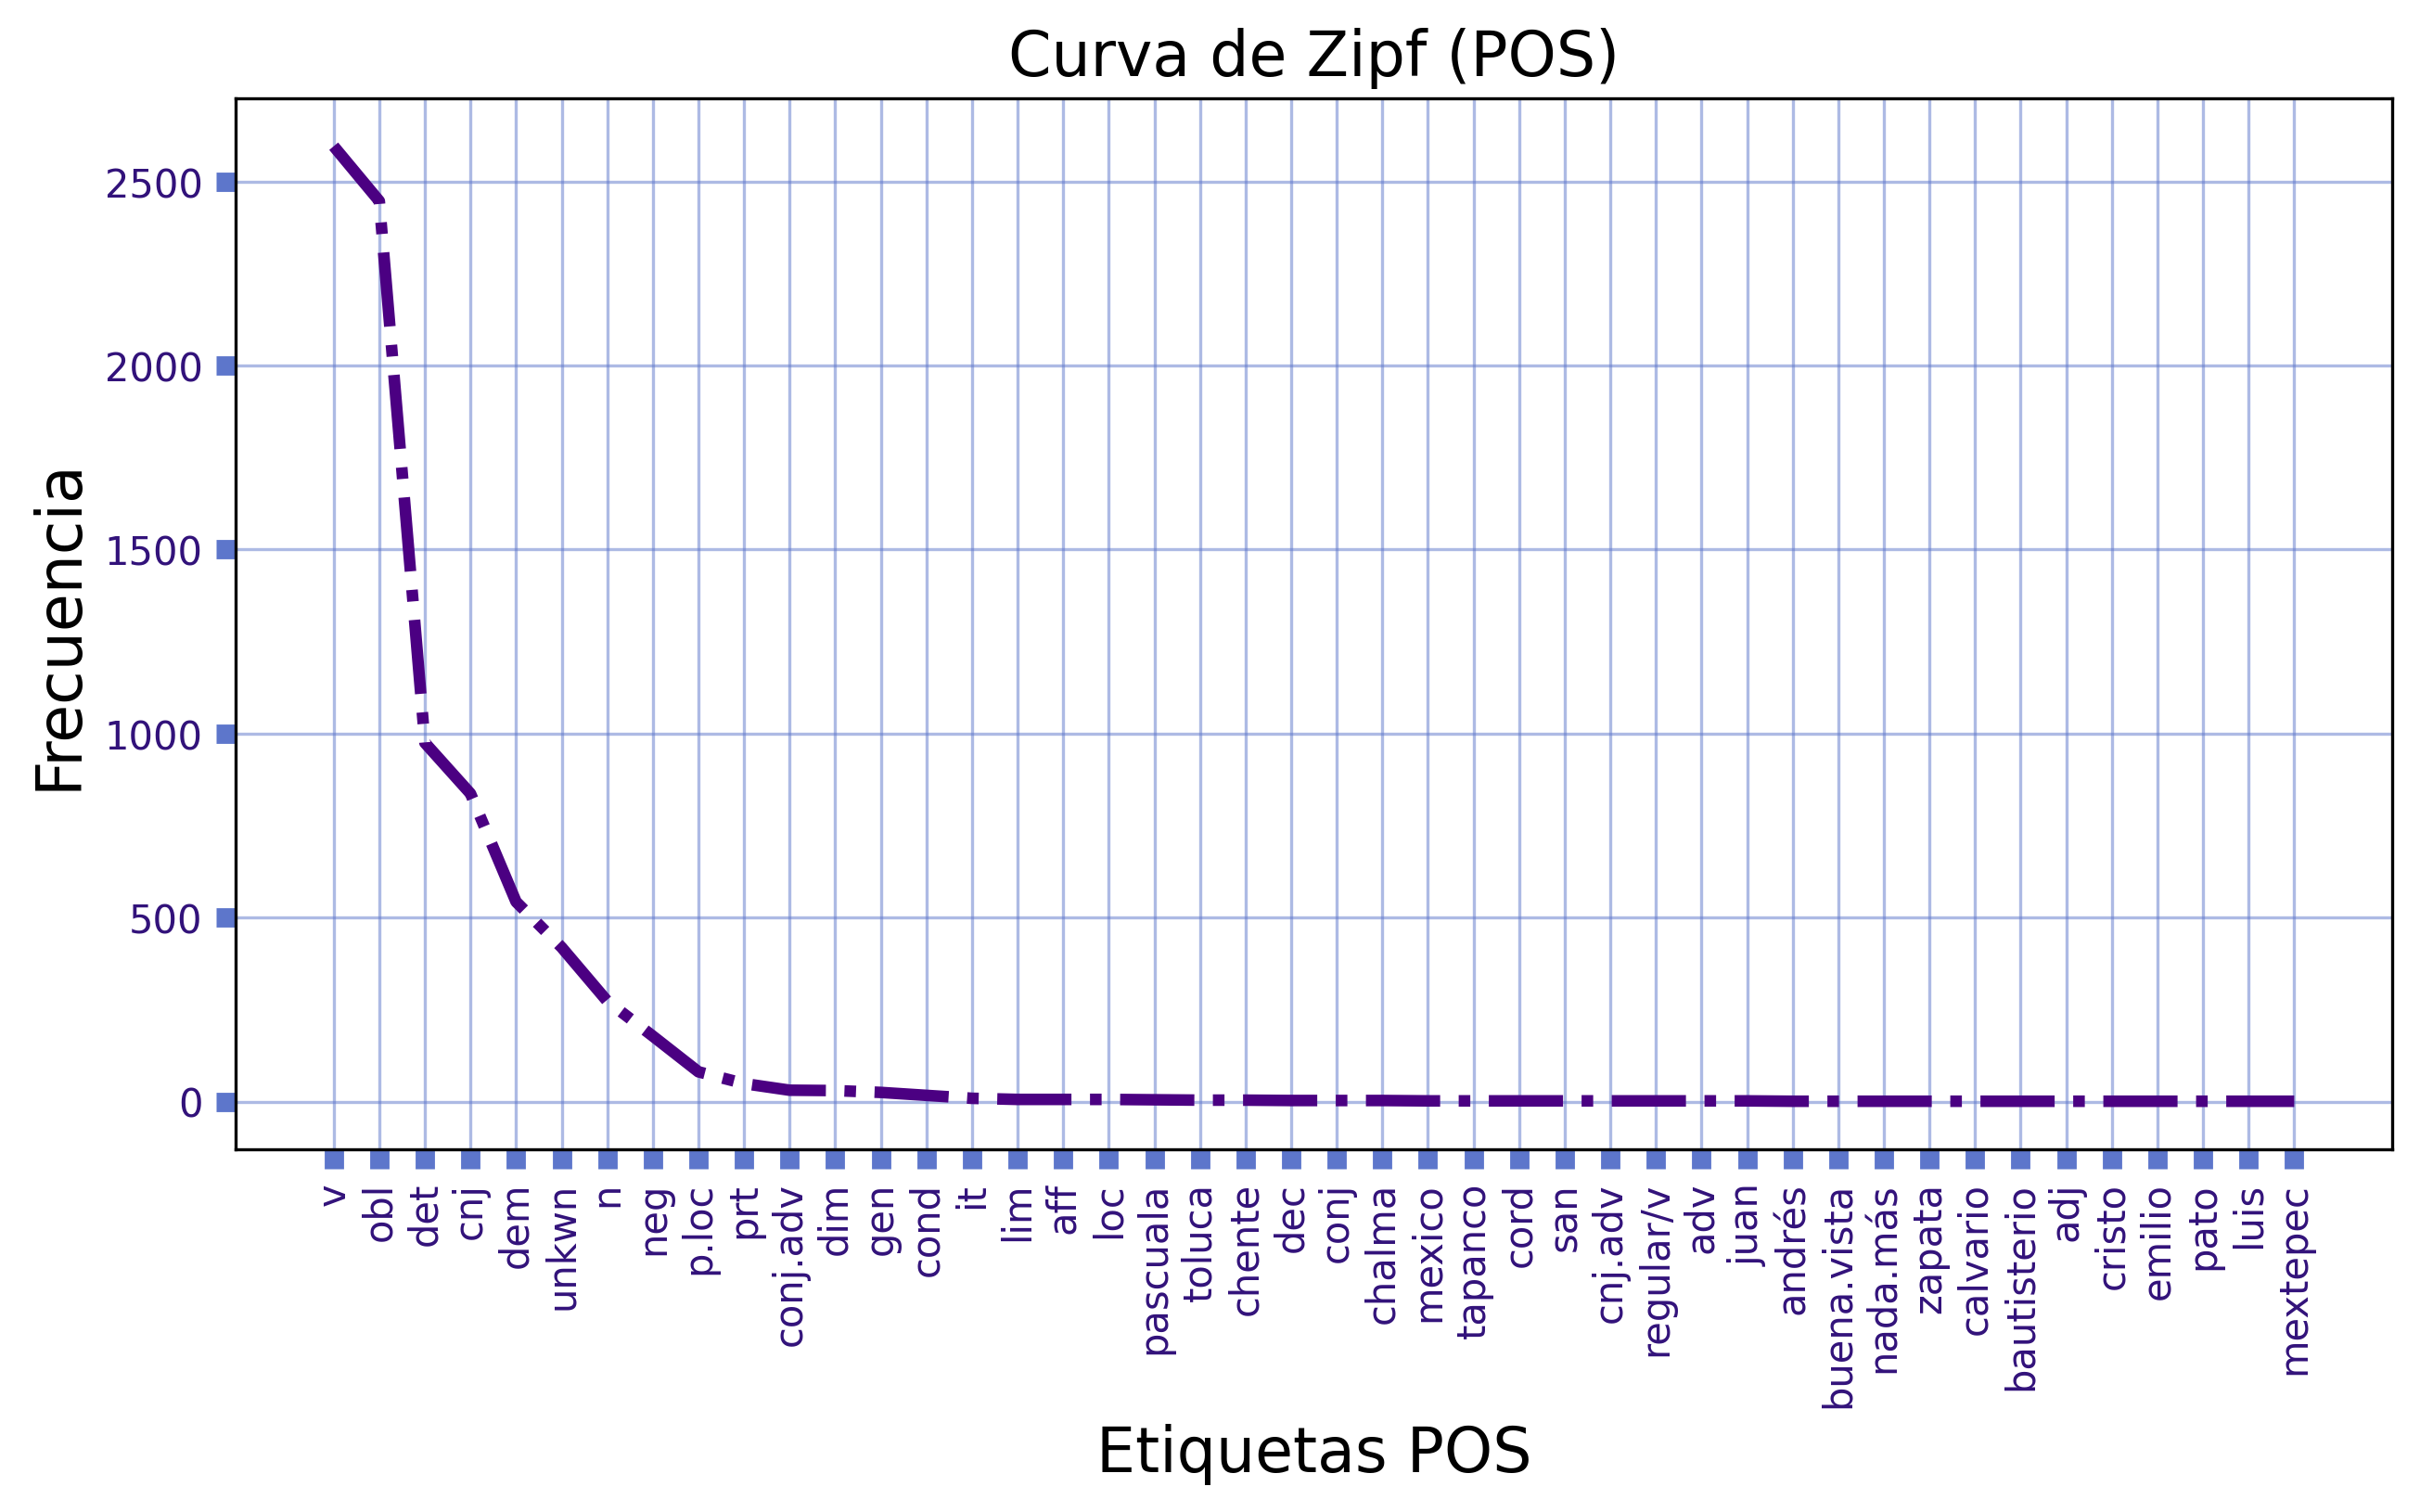
\includegraphics[width=\textwidth]{zipf_pos}
	\caption{Distribución de etiquetas POS}
\end{figure}

\begin{figure}[h]
	\centering
	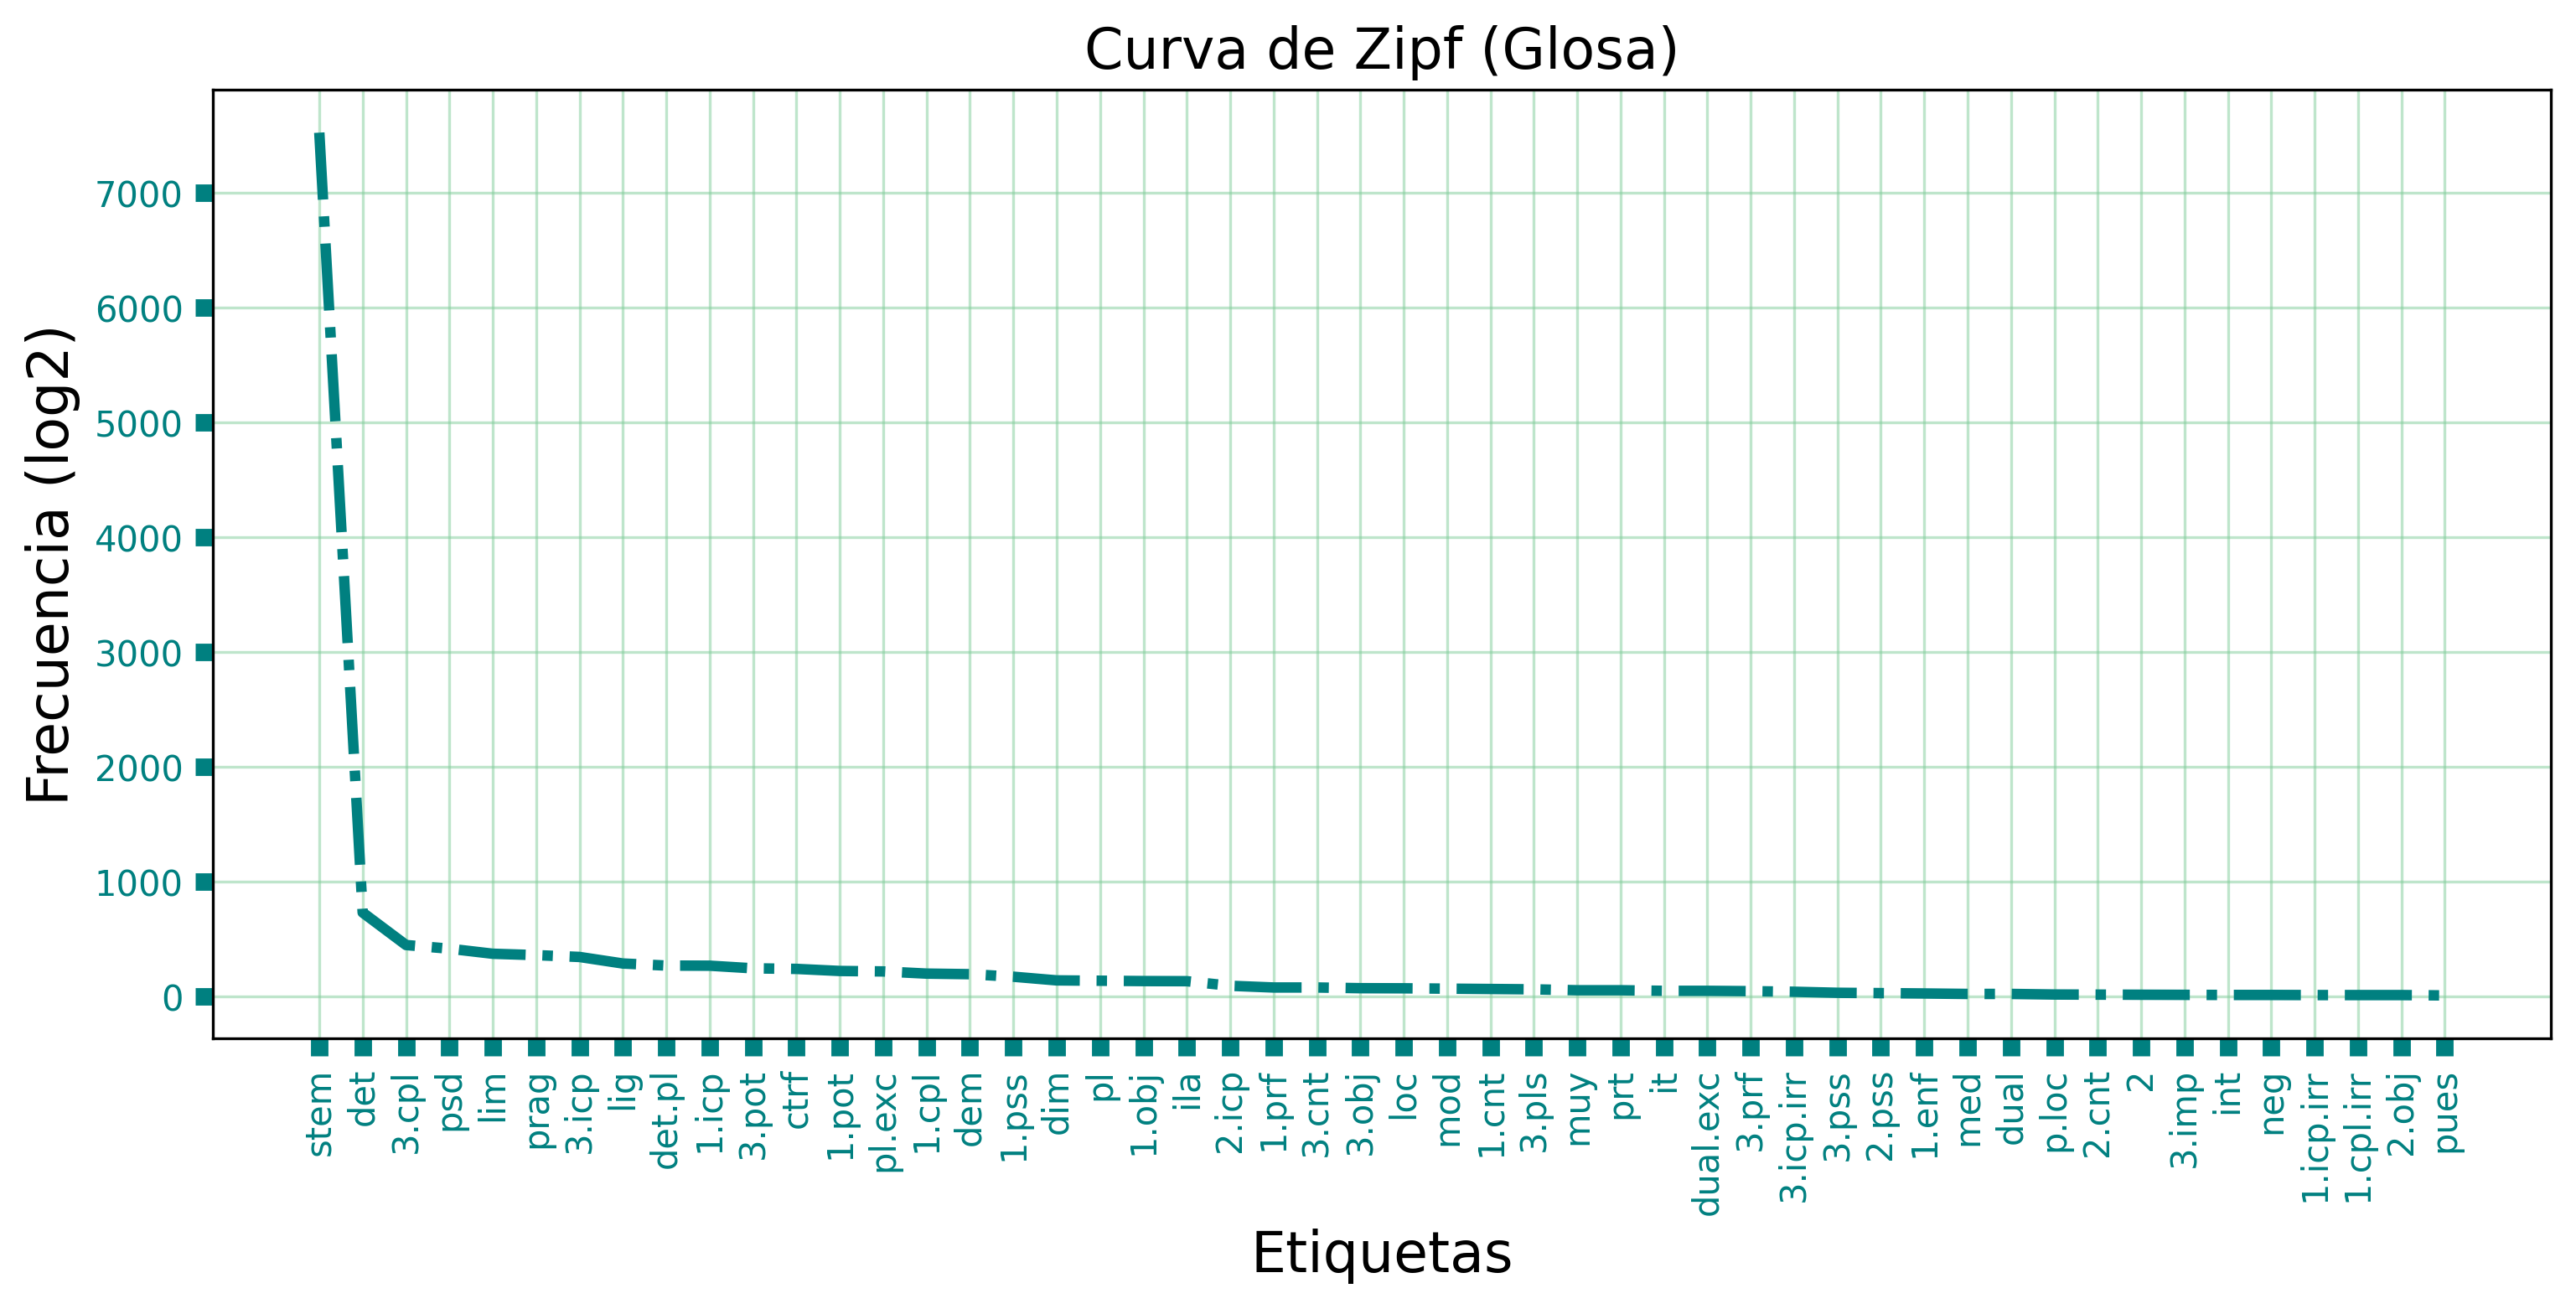
\includegraphics[width=\textwidth]{zipf_gloss}
	\caption{Distribución de glosa (primeras 50)}
\end{figure}

\begin{figure}[h]
	\centering
	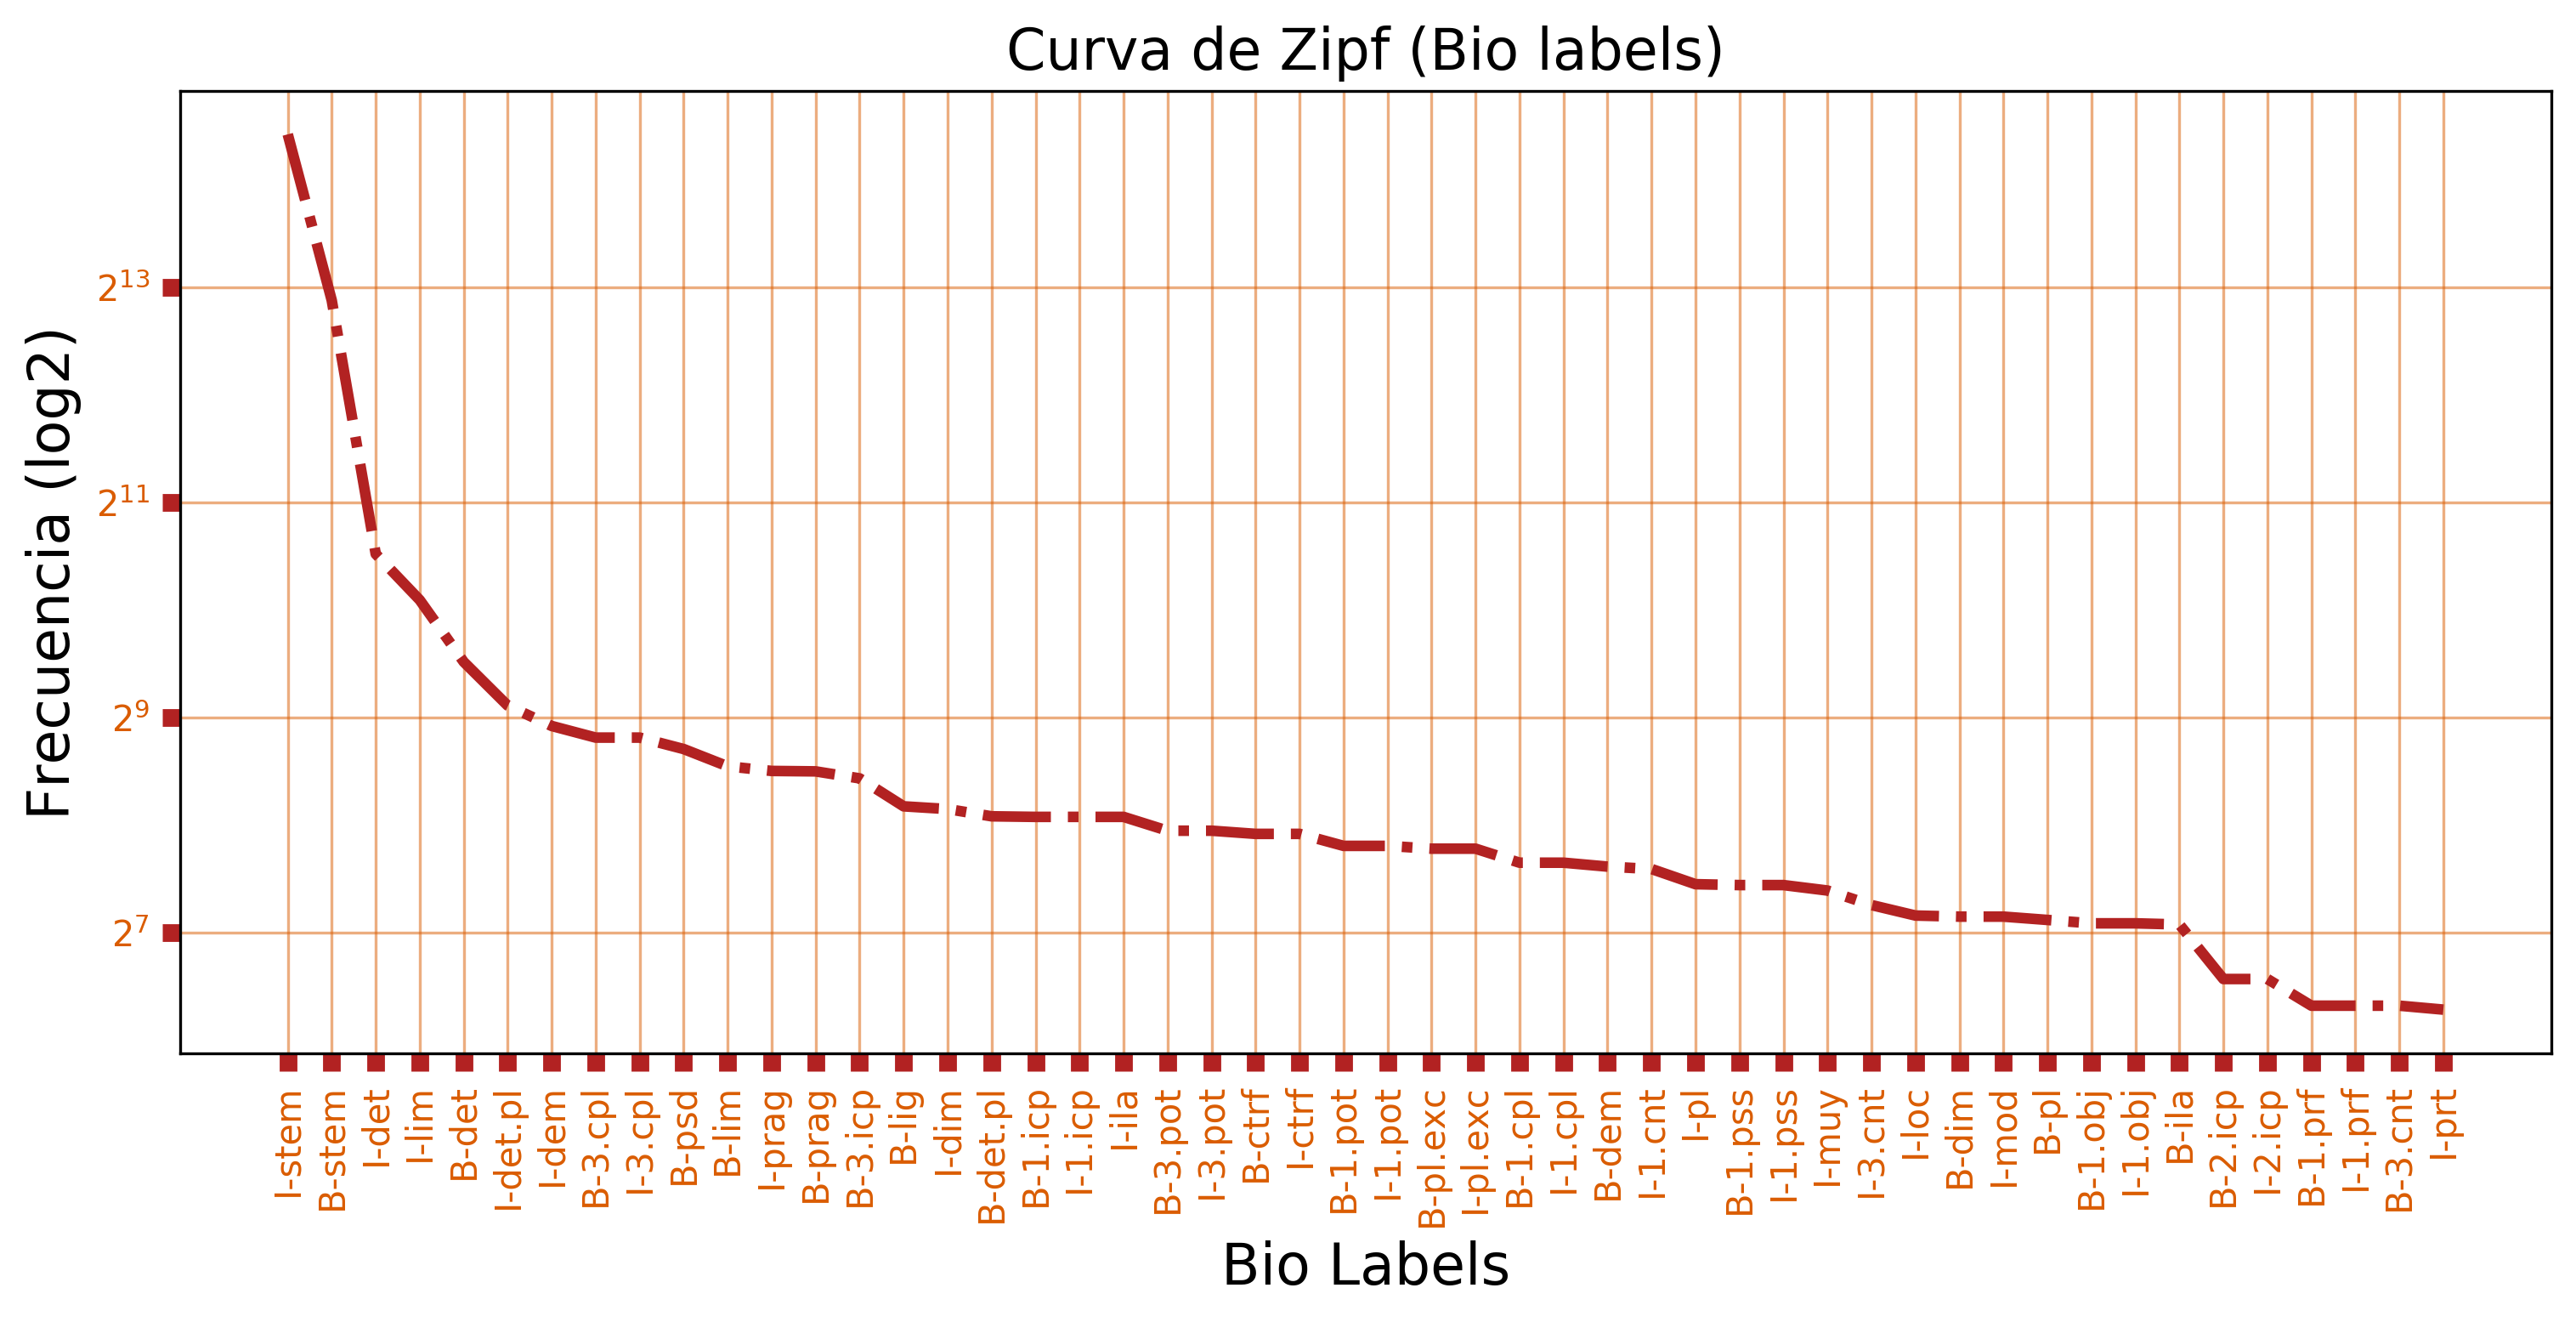
\includegraphics[width=\textwidth]{zipf_bio}
	\caption{Distribución de Bio Labels (primeras 50)}
\end{figure}

%4. Numero de etiquetas diferentes
%5. Tipos de POS y cuantos de cada uno

%Descripción general del corpus. Orientar que la arquitectura esta enfocada en
%resolver el problema de low resources

\section{Arquitectura}

Para esta tesis proponemos una arquitectura de aprendizaje
estructurado  supervisado utilizando un método gráfico, Conditional
Random Field (CRF), que permitirá la predicción de secuencias que describen
las unidades morfológicas (glosa) dentro de una palabra en otomí

Se utilizaron CRFs para predecir secuencias de glosa, que será la salida $Y$
dadas las observaciones $X$ que son el texto previamente glosado. Puntualmente,
se utiliza el modelo gráfico 1st-order Markov CRF with dyad features.
Adicionalmente, es utilizado el algoritmo de aprendizaje de Limited-memory
Broyden-Fletcher-Goldfarb-Shanno (L-BFGS) como se menciono en TODO.

Con base en el trabajo previo para del idioma Lezgi \citep{moeller2018automatic} se plantea como hipótesis que dado el tamaño del corpus y la glosa que contiene
se obtendrá texto correctamente glosado con una precisión de al menos 80\%. El objetivo de esta arquitectura es obtener al menos un TODO\% de precisión
Ya que el resultado esperado es la generación de etiquetas que, en principio,
dependen unas de otras un método basado en grafos como los CRF puede ser
adecuado. Se definieron de aprender un conjunto de feature functions que
describen TODO el contexto y brindan información útil para la fase de
entrenamiento.

El modelo de aprendizaje semi-supervisado, para la generación de glosa para
el otomí se describe a continuación:

HACER ESTA PARTE POR PUNTOS MAS BREVES Y CADA PUNTO HACERLO SECCION Y PROFUNDIZAR

\begin{itemize}
	\item Obtener el corpus en otomí previamente glosado y obtenerlo en un
	formato que especifique la información de las oraciones a nivel
	de letra especificando su Bio Label.
	\item Los CRF toman como entrada los datos $X$ que corresponden al
	corpus en otomí introducido en las feature functions asociados
	de forma biyectiva con la etiqueta Bio Label que le corresponde.
	Con base en esto se entrenará un modelo que busque maximizar el
	logaritmo de verosimilitud con el método de aprendizaje L-BFGS
	\item Posterior se obtendrá un modelo entrenado con el que se generarán
	etiquetas de glosa para el otomí. Por lo tanto, el modelo
	recibirá párrafos de texto en otomí y retornará el texto
	glosado.
	\item Se considera exitosa la predicción si se logra maximizar la
	correcta clasificación de las secuencias de salida. Para
	determinar si la predicción fue exitosa se utilizaron técnicas
	típicas de ML como K-folds que consiste en tomar K fragmentos
	de los datos de entrada para utilizarlos para probar el modelo
	y asi obtener una precisión, recall y F-score.
\end{itemize}

% Definir el metodo en funcion del marco teorico
% ¿Que es X y Y?
% Feature functions
% Como se decidieron
% ¿Porque estas caracteristicas son reelevantes?
% Que es para nosotrxs una FF
% Experimentos quitando features functions
% Diagram de donde se encuentran estos elementos en la arquitectura
% Como se calculan lambdas y mu
% Variacion de hiperparametros
% Descripcion de que variaciones se hicieron

% Resumen al final (pasos de todo lo que se hizo)

MENCIONAR python, versión, paquetes y donde corrio. En promedio cuanto tarda
en correr en la maquina. Mencionar el original en c++

\section{Feature functions}

\chapter{Experimentación y Resultados}

Cualitativos y cuantitativos

Hablar del Base line y como mejoró con mas features

\section{Corpus de evaluación}

Aquí se habla del K fold y de como se introdujo el corpus retador( ,

\citet{singh2005comparison}

\section{Análisis de resultados}

\chapter{Conclusiones}

\bibliography{tesis}
	
\end{document}